\newpage
\begin{center}
  \textbf{\large 2. АНАЛИЗ НАБОРОВ ПОСЛЕДОВАТЕЛЬНОСТЕЙ}
\end{center}
\refstepcounter{chapter}
\addcontentsline{toc}{chapter}{2. АНАЛИЗ НАБОРОВ ПОСЛЕДОВАТЕЛЬНОСТЕЙ}

\section{Расширение алгоритма PCA-Seq для анализа наборов последовательностей}

До этого момента мы рассматривали алгоритм PCA-Seq исключительно для анализа отдельных последовательностей. Однако гораздо чаще в практике встречаются случаи, когда нам необходимо анализировать несколько последовательностей, сравнивать их между собой, использовать, как исходные данные для задач классификации и регрессии. При этом часто последовательности имеют разную длину, что усложняет применение к ним классических методов предобработки данных или делает их менее эффективными.

Идея нашего метода заключается в повторном применении шагов алгоритма PCA-Seq, тем самым делая возможным анализ нескольких последовательностей. Рассмотрим подробнее, что подразумевается под повторным применением шагов.

Напомним, что при анализе отдельных последовательностей в качестве результата алгоритма мы получаем фазовую траекторию исходной последовательности в пространстве главных компонент. Пример можно увидеть на рисунке~\ref{trajectory} из предыдущей главы.

Пусть мы рассматриваем $Q$ последовательностей $S_1,\ldots,S_Q$ длины \\$K_1,\ldots,K_Q$ соответственно, и по каждой из них проходим скользящим окном с общими фиксированными параметрами $W$ и $T$. Для каждой последовательности получаем $N_i~= \left\lceil\frac{K_i-W}{T}\right\rceil + 1$ фрагментов ($F_{i1},\ldots, F_{iN_i}$). Всего $N = N_1 + \ldots + N_Q$ фрагментов.

Применив PCoA к множеству фрагментов, полученных из всех последовательностей и соединив в нужном порядке точки, относящиеся к одним и тем же последовательностям, мы получим несколько фазовых траекторий, расположенных в общем евклидовом пространстве главных компонент.

Пусть точка $X_{ij}$ соответствует фрагменту $F_{ij}$ ($i \in \{1,\ldots, Q\}$, \\$j \in \{1, \ldots, N_i\}$). Тогда получаем фазовые траектории:

\begin{itemize}
  \item $\hat{T}_1 = X_{11},\ldots,X_{1 N_1}$,
  \item $\hat{T}_2 = X_{21},\ldots,X_{2 N_2}$,
  \item $\ldots$
  \item $\hat{T}_Q = X_{Q1},\ldots,X_{Q N_Q}$.
\end{itemize}

Уже на этом этапе мы получаем наглядное геометрическое представление набора молекулярных последовательностей. Каждая последовательность представляется ломаной, при этом близкие друг другу фрагменты (согласно выбранной метрике) отображаются в близкие друг другу точки, а длины получившихся ломаных пропорциональны длинам исходных последовательностей.

Однако мы можем получить представление последовательностей и в виде точек. Введем метрику $d_T(\hat{F}_i, \hat{F}_j)$, которая будет считать расстояние между фазовыми траекториями (ломаными) разной длины. Тогда мы можем построить матрицу расстояний между фазовыми траекториями и применить к ней PCoA. Тем самым мы получим геометрическое представление для каждой из исходных последовательностей в виде точки в пространстве главных компонент.

\section{Выбор метрик для расчета расстояний между фазовыми траекториями}

\section{Задача предсказания термофильности организмов}

\begin{figure}[!t]
  \centering
  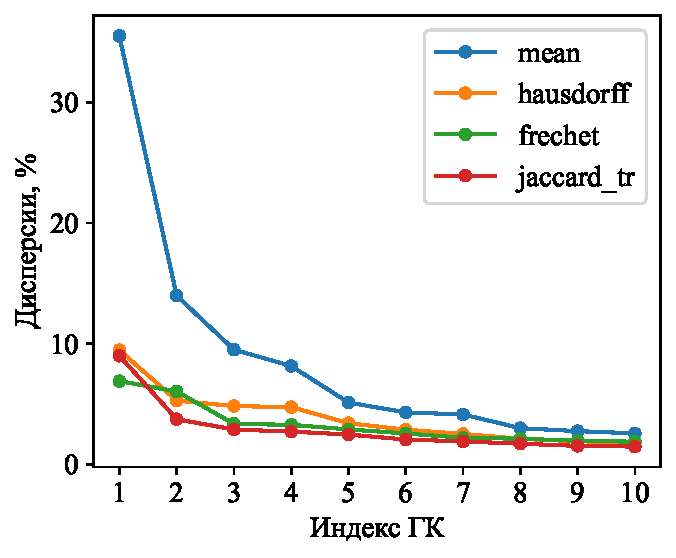
\includegraphics{dispersions-tr.pdf}
  \caption{Распределения дисперсий первых десяти главных компонент для различных метрик между фазовыми траекториями}
  \label{dispersions-tr}
\end{figure}

\section{Результаты применения метода}
